%%%%%%%%%%%%%%%%%%%%%%%%%%%%%%%%%%%%%%%%%%%%%%%%%%%%%%%%%%%%%%%%%%%%%%%%%%%%%%%%%%%%
The COVID-19 pandemic, with its severity of diseases and contagability, indicates
how great of a need there is for accurate and fast modeling methods. In this thesis, I demonstrate a model that incorporates the spatial spread of viruses and produces accurate simulations in a few seconds or minutes, so that the model can be used to study viruses in a more accurate way. 

\section{Basic Virology}
Viruses are microscopic parasites, generally much smaller than bacteria, that lack the capacity to thrive and reproduce outside of a host body \citep{website2}. A virus is composed of a nucleic acid genome and a protein capsid that covers the genome \citep{website3}. As seen in figure \ref{fig:Virus_Replication}, the life cycle of a virus begins with the virus attaching to or being absorbed by the host cell. Once the virus genome enters into a cell, the genome moves to the ribosomes, where the genome is replicated. After the genome is replicated, new virus can be assembled and released from the host cell \citep{Kaiser}, allowing the virus to continue spreading through out the host cells. \color{red} I think you're better off citing a virology textbook at the end of the paragraph instead of citing a bunch of different websites throughout.\color{black}

\begin{figure}[h]
    \centering
    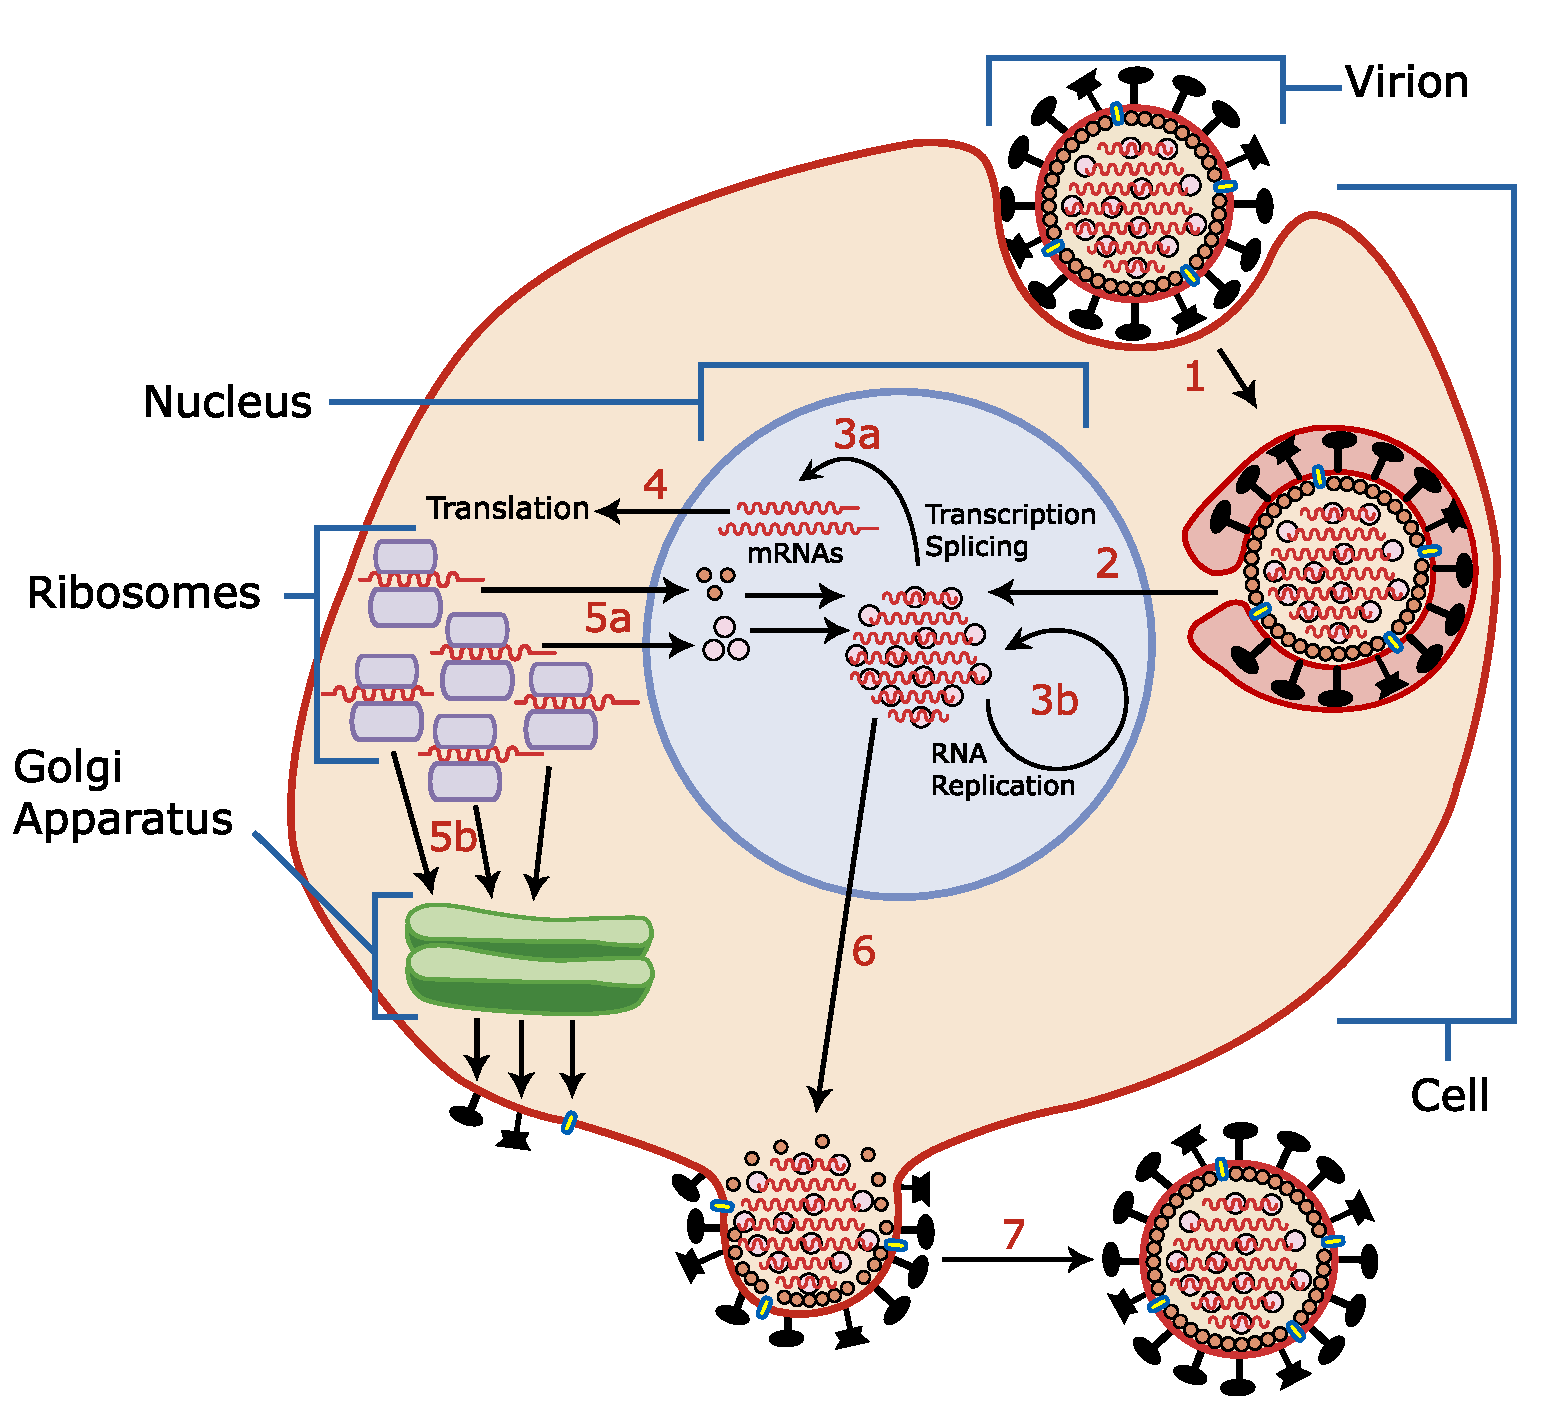
\includegraphics[width=0.6\linewidth]{Figures/Virus_Replication_large.pdf}
    \caption{The life cycle of a virus begins with a virion (virus particle) being absorbed by the cell. Once the virion enters into a cell the virus genome is released. The genome moves to the ribosomes, where the genome is replicated. With the replicated genome, new virus can be assembled by the golgi apparatus and then released from the cell.}
    \label{fig:Virus_Replication}
\end{figure}

Some viruses cause illnesses and a few of them are severe enough to cause global pandemics: the 2019-2021 coronavirus pandemic (a widespread global outbreak), the 2014 outbreak of Ebola in West Africa, and the 2009 H1N1/swine flu pandemic, for example. Other viruses, like influenza, are endemic or cause seasonal outbreaks. In total, the Centers for Disease Control and Prevention (CDC) estimates that in the United States up to 42.9 million people were sick during the 2018-2019 flu season, 647,000 people were hospitalized, and 61,200 died \citep{website4}. \color{red} The CDC probably has the stats published in the Morbidity and Mortality Weekly Report (MMWR), so find that and use it as a citation. \color{black}

In order to understand viruses, assays are performed. An assay is an experiment for assessing or measuring characteristics of a substance. The two typical forms of assays are quantitative and quantal. Quantitative assays are assays that give an accurate and exact measure of the amount of a substance in a sample. Of these types of assays, plaque assays are the most widely used for determining viral titer \citep{Kumar}. They can be used with any virus that causes damage to the cells where they have been grown. This damage is called a plaque and is roughly circular in shape. These assays are often performed in petri dishes or multi-well plates with a small number of wells, where virus is placed in a dish/well of healthy cells and the formation of plaques and the concentration of virus are monitored. It is assumed that each plaque formed is caused by one virus particle. Because of this assumption, the viral concentration is often recorded as plaque forming units per milliliter (pfu/mL). Quantal assays are assays which generally give only a pass or fail. These assays are performed in many mediums such as in animals or multi-well plates. Any virus that will infect the medium can be used. When multi-well plates are used, different groups of wells on the plate are filled with a dilution of virus that often varies in a ten fold difference from group to group. After a set amount of time the wells are observed for a reaction, and whether or not a well has a response is counted. When animals are used, different animal subjects are injected with a dilution of virus that often varies in a ten fold difference from subject to subject. After a set amount of time the animals are observed, and whether or not an animal shows symptoms or dies is counted.


When studying a virus, \emph{in vitro} viral infection assays are performed on a monolayer of cells grown in a petri dish or a multi-well plate. These dishes and plates are a type of adherent culture where the cells are grown on a nutritious substrate. When the cells are grown to confluence the cells tend to push on each other and distort the shape of each cell membrane \citep{bruckner_importance_2018} \color{red}The name on this reference is misspelled\color{black}. When \emph{in vitro} viral infections are performed on the layer of cells, there is on the order of \numrange[range-phrase = --]{e5}{e6} cells in the dish or well \citep{Number_of_cells_in_a_dish_noauthor_useful_nodate}. 

%%%%%%%%%%%%%%%%%%%%%%%%%%%%%%%%%%%%%%%%%%%%%%%%%%%%%%%%%%%%%%%%%%%%%%%%%%%%%%%%%%
\section{Modeling of assays}

Virus modelers are using ABMs to simulate the two dimensional layer of agents to replicate experiments that are done \emph{in vitro} in order to better understand factors that affect viral spread. The agent-based model framework is appealing to virus modelers because it allows for the individual tracking of how cells, as agents, interact with the virus, and has the potential to replicate \emph{in vitro} and eventually \emph{in vivo} viral infections. Currently, however, the implementation of agent-based models in the field of virology has two issues: speed and size. 


In recent years, the field of virology has started using agent-based models to study the spread of viruses during a viral infection assay \citep{beauchemin_simple_2005,alvarado_cellular-level_2018,wodarz_laws_2014,tong_development_2015,whitman20,goyal16,itakura10,wasik14} in an effort to study the spatiality of viral spread. Agent-based (individual-based or micro-simulation) models have been around since 1970 with the introduction of ``Conway's Game of Life'' \citep{gardner70}. These models have been utilized in many different fields from physics to the study of fish (ichthyology) \citep{owusu20} and continue to be popularized for different applications by software like Netlogo \citep{nogare20,chiacchio14}. The models consist of a collection of agents whose behavior is determined by mathematical or computational rules. The agents of the system can move freely \citep{beauchemin07} or be fixed in a grid or lattice \citep{beauchemin_simple_2005} for varying applications, but either configuration allows for tracking of spatially emergent patterns. 

Virus modelers are using ABMs to simulate the two dimensional layer of agents to replicate experiments that are done \emph{in vitro} in order to better understand factors that affect viral spread. The agent-based model framework is appealing to virus modelers because it allows for the individual tracking of how cells, as agents, interact with the virus, and has the potential to replicate \emph{in vitro} and eventually \emph{in vivo} viral infections. Currently, however, the implementation of agent-based models in the field of virology has two issues: speed and size. 

Agent-based models are notorious for being computationally intensive and taking long amounts of time to run simulations. This point has been commented on in a previous article \citep{gallagher_causes_2018} and the feasibility of ABMs for research has been talked about as a goal that is to come with increasing computational advancements \citep{bauer_agent-based_2009}. Previous research has addressed this lack of computing power issue by reducing the number of agents modeled and therefore reducing the number of computations required for a simulation. The number of agents published is at minimum an order of magnitude lower then the number of target cells used in the corresponding experimental data. Beauchemin et al.\ \citep{beauchemin_simple_2005} simulated \num{1.232e5} agents, while the experiment they were attempting to replicate was performed in 6 well-plates and had $\sim$\num{1.2e6} cells per well. Alvarado et al.\ \citep{alvarado_cellular-level_2018} simulated \num{4.0e4} agents when trying to replicate experiments also performed in 6 well-plates. Wodarz et al.\ \citep{wodarz_laws_2014} simulated \num{2.0e4} agents, while the experiment they were replicating was performed in 24 well-plates and had $\sim$\num{2.4e5} cells per well. Tong et al.\ \citep{tong_development_2015} simulated \num{6.0e5} agents in an effort to simulate mice lungs, which have $\sim$\num{e9} cells. These smaller simulations are more affected by boundary interactions, which can result in model dynamics that don't faithfully reproduce the infection. Having an in-host model that can produce accurate simulations in a timely manner not only allows for the prediction of patient infection, but also can be used to flush out potential causes of varying symptoms in patients. 

%%%%%%%%%%%%%%%%%%%%%%%%%%%%%%%%%%%%%%%%%%%%%%%%%%%%%%%%%%%%%%%%%%%%%%%%%%%%%%%%%%
\section{Exigence}
While it might be feasible to wait long periods of time to run accurate simulations for endemic or recurrent seasonal viruses, recent events of the COVID-19 pandemic indicate how great a need there is for accurate and fast modeling methods. Epidemiological population-level modeling tools that include both ordinary differential equation (ODE) models \citep{li20,ngonghala20} and ABMs \citep{ying21,sneppen21,kano21} were immediately deployed to help predict how the new virus would spread around the world and how different interventions could help stem the spread. At the within-host level, the primary modeling tool was limited to simple ODE models \citep{goncalves20,wang20model,hernandez20,dogra20} that lack the ability to reproduce the spatial heterogeneity of real viral infections. Fast and accurate in-host models could be helpful in assessing the potential of re-purposed drugs \citep{czuppon21,goncalves20,dodds20}, finding indicators of disease severity or mortality \citep{neant21}, and assessing the effectiveness of testing \citep{ejima21}. A community-driven ABM incorporating many realistic biological responses was quickly developed for SARS-CoV-2 \citep{getz21}, but is only currently simulating a few thousand agents and is expected to need high-performance computing or cloud resources to parameterize the model. Thus, there is a need to develop modeling and simulation tools for accurately predicting in-host viral dynamics that can be quickly deployed to help combat the next pandemic.

%%%%%%%%%%%%%%%%%%%%%%%%%%%%%%%%%%%%%%%%%%%%%%%%%%%%%%%%%%%%%%%%%%%%%%%%%%%%%%%%%
\section{Scope}

In this work, the testing, validation, and application of a hybrid ABM and PDM implemented on GPUs is presented. The work here begins with the methods where the four attributes of the model, the agent-based model of the cells, the partial differential equation of the virus, the cell-free transmission mode of viruses, and fitting of the model to data, are explained.  Then, the results of model implementation with parallel programming, convergence testing, and simulation speed improvement are presented. Next, we show that the model can reproduce experiments by fitting the model to an example data set from an \emph{in vitro} influenza experiment. Finally, it is shown how the model can be used to make measurements of viral titter curves to study inoculum-dependence in SARS-CoV-2 infection severity. This work shows how an ABM/PDM hybrid model of in-host infections is ensured to numerically converge, be applied to experimental data for parameter extraction, and produce simulations with in seconds to minutes for timely application. It will also be shown that from the simulations different characteristics of viral titer curves can be measured to gain insight on severity of viral infections. \color{red} I don't think you need to list all the things you're not doing. Take out the next sentences \color{black}. At this moment, the work will not compare in detail past models (ODE, ABM, etc...) with the proposed model. It will only look at experimental systems that are petri dishes or quantitative multi-well plates. The work will not compare full project times or costs when using high performance computers vs desktop GPU accelerated code. Finally, the work will not compare two dimensional numerical integrator schemes of PDEs.




